\documentclass[10pt,twocolumn,a4paper]{article}
% Kompilacja: pdfLaTeX + BibTeX (latexmk -pdf raport_etap1.tex).
% Liczby oznaczone makrami (\TestAuc itd.) pochodzą z pliku wyniki.tex,
% generowanego przez notatnik 4_etap1_model.ipynb.
\usepackage[T1]{fontenc}
\usepackage[utf8]{inputenc}
\IfFileExists{polski.sty}{\usepackage{polski}}{%
  % awaryjnie, gdy w instalacji TeX-a brakuje pakietu polski
  \AtBeginDocument{\renewcommand{\figurename}{Rysunek}\renewcommand{\tablename}{Tabela}%
  \renewcommand{\contentsname}{Spis treści}}}
\usepackage{lmodern}
\usepackage[margin=18mm,columnsep=7mm]{geometry}
\usepackage{microtype,graphicx}
\usepackage{booktabs,tabularx,array}
\usepackage{amsmath,amssymb}
\usepackage{enumitem,placeins,xcolor,xurl,float,needspace,etoolbox}
\usepackage[hidelinks,breaklinks=true]{hyperref}
\hypersetup{pdftitle={Speed Dating Experiment -- raport projektowy, etap 1}}
\setlist[itemize]{leftmargin=*,itemsep=1pt,topsep=3pt}
\setlist[description]{leftmargin=0pt,labelsep=4pt,itemsep=3pt}
\setlength{\emergencystretch}{1em}
\raggedbottom
\pretocmd{\section}{\Needspace{6\baselineskip}}{}{}
\pretocmd{\subsection}{\Needspace{5\baselineskip}}{}{}
\newcolumntype{Y}{>{\raggedright\arraybackslash}X}
\renewcommand{\abstractname}{Streszczenie}
\renewcommand{\refname}{Bibliografia}

% Plik generowany automatycznie przez 4_etap1_model.ipynb – nie edytować ręcznie.
\newcommand{\NTrain}{3296}
\newcommand{\NTest}{888}
\newcommand{\MatchTrain}{16{,}7}
\newcommand{\MatchTest}{15{,}7}
\newcommand{\NCech}{123}
\newcommand{\NDuplikaty}{19}
\newcommand{\ValAucMean}{0{,}588}
\newcommand{\ValAucStd}{0{,}045}
\newcommand{\TestAuc}{0{,}571}
\newcommand{\TestAp}{0{,}202}
\newcommand{\TestBacc}{0{,}562}
\newcommand{\TestFone}{0{,}289}
\newcommand{\TestAcc}{0{,}528}
\newcommand{\DummyAuc}{0{,}482}
\newcommand{\DummyFone}{0{,}132}
\newcommand{\AlwaysNoAcc}{0{,}843}
\newcommand{\ForestAucMean}{0{,}574}
\newcommand{\ForestAucStd}{0{,}015}
\newcommand{\CurveFirst}{0{,}526}
\newcommand{\CurveLast}{0{,}594}

\newcommand{\TematProjektu}{Speed Dating -- czy będzie obustronna sympatia?}
\newcommand{\TypZadania}{klasyfikacja binarna (match / brak matcha)}

\title{\TematProjektu\\[2mm]
\large Zaawansowane metody uczenia maszynowego -- raport, etap~1}
\author{Jakub Balicki\\\small Numer albumu: 148889\\\small Informatyka II st., Data Science, grupa DS1}
\date{18 listopada 2026}
\begin{document}
\maketitle

\begin{abstract}
Na danych z~eksperymentu speed dating sprawdzam, czy da się przewidzieć,
że po kilkuminutowej rozmowie obie osoby zechcą spotkać się ponownie (\emph{match}).
Korzystam tylko z~informacji znanych przed rozmową, czyli z~ankiet wypełnionych
przy zapisie. Match zdarza się w~ok.\ 16\% spotkań. W~etapie~1 przygotowałem dane,
porównałem pięć metod uzupełniania braków i~zbudowałem prosty model bazowy
(regresja logistyczna bez strojenia). Na zbiorze testowym osiąga on ROC AUC =
\TestAuc{} (model losowy: \DummyAuc{}). Model jest więc lepszy od losowania, ale słaby,
co pokrywa się z~wynikami innych badań.
\end{abstract}

\section{Problem, motywacja i cel}
\subsection{Pytanie predykcyjne}
Organizator randek w~formule speed dating chciałby z~góry wiedzieć, które pary mają
największą szansę na obustronną sympatię, np.\ żeby lepiej układać kolejność rozmów.

\noindent\textbf{Typ zadania:} \TypZadania.

\noindent\textbf{Kontrakt predykcji:} jednostka -- jedno spotkanie kobiety i~mężczyzny;
moment -- przed rozmową; cechy -- ankiety obu osób z~zapisu (wiek, rasa, kierunek
studiów, zainteresowania, czego szukają u~partnera) i~informacje o~wydarzeniu;
cel -- \texttt{match} = 1, gdy obie osoby powiedziały ,,tak''.

\subsection{Kryterium użyteczności}
Model ma sens, jeśli szereguje pary lepiej niż losowo (ROC AUC wyraźnie powyżej 0,5).
Samo accuracy nie wystarczy: model, który zawsze mówi ,,brak matcha'', ma na teście
accuracy \AlwaysNoAcc{}, a do niczego się nie przydaje.

\section{Dane i analiza wstępna}
\subsection{Źródło i znaczenie kolumn}
Zbiór \emph{Speed Dating Experiment} z~Kaggle (\texttt{annavictoria/speed-dating-experiment}),
zebrany przez Fismana i~in.~\cite{fisman2006} na Columbia University w~latach 2002--2004.
Ma 8378 wierszy i~195 kolumn. Jeden wiersz to decyzja \emph{jednej} osoby po jednej
rozmowie. W~21 wydarzeniach (falach) wzięło udział 551 osób, co daje 4184 spotkania.

Wiersze kobiety i~mężczyzny z~tego samego spotkania połączyłem w~jeden wiersz.
Usunąłem kolumny wypełniane po rozmowie (np.\ oceny partnera po spotkaniu, ankiety
z~kolejnych tygodni), bo przed rozmową ich nie znamy, a ich użycie zawyżyłoby wynik.

\begin{table}[H]
\centering
\caption{Najważniejsze kolumny (końcówki \texttt{\_woman}/\texttt{\_man} oznaczają osobę w~parze).}
\label{tab:dane}
\footnotesize
\begin{tabularx}{\columnwidth}{@{}lYl@{}}
\toprule
Kolumna & Znaczenie & Typ\\
\midrule
\texttt{age} & wiek [lata] & liczbowa\\
\texttt{race}, \texttt{samerace} & rasa; czy ta sama w~parze & nominalna\\
\texttt{field\_cd}, \texttt{career\_c} & kierunek studiów, kariera (kody) & nominalna\\
\texttt{goal} & po co ktoś przyszedł & nominalna\\
\texttt{date}, \texttt{go\_out} & jak często randkuje / wychodzi (1--7) & porządkowa\\
\texttt{sports} \dots\ \texttt{yoga} & zainteresowania (1--10) & porządkowa\\
\texttt{int\_corr} & podobieństwo zainteresowań pary & liczbowa\\
\texttt{attr1\_1} \dots & czego szuka u~partnera (100 pkt) & liczbowa\\
\texttt{income} & średni dochód w~okolicy zamieszkania & liczbowa\\
\texttt{match} & oboje powiedzieli ,,tak'' & cel\\
\bottomrule
\end{tabularx}
\end{table}

\subsection{Jakość i struktura danych}
\textbf{Klasy:} match ma \MatchTrain\% spotkań w~zbiorze treningowym i~\MatchTest\%
w~testowym, więc klasy są niezbalansowane.

\textbf{Braki:} brakuje ok.\ 6\% wartości, ale prawie każdy wiersz ma jakiś brak.
Najwięcej braków mają dochód, czesne i~wyniki SAT uczelni (40--60\%).
Kolumny z~ponad 60\% braków usunąłem.

\textbf{Błędy:} literówki w~tekstach (np.\ \emph{finanace}), liczby zapisane jako tekst
z~przecinkami, kilka osób, którym punkty preferencji nie sumują się do 100. Największy
problem: w~falach 6--9 jedno pytanie (,,czego szukają inni'') zebrano w~skali 1--10
zamiast rozdania 100 punktów. Przeliczyłem te odpowiedzi na udziały, żeby wszystkie
fale miały tę samą skalę.

\textbf{Typy danych:} kolumny nominalne zamieniam na kolumny 0/1 (one-hot), porządkowe
zostawiam jako liczby. Znaczników czasu w~danych nie ma (\texttt{wave} to numer
wydarzenia, a~\texttt{date} to częstość randek). Duże dochody nie są błędem, więc
ich nie usuwam, tylko biorę logarytm.

\subsection{Najważniejsze obserwacje z EDA}
Rysunek~\ref{fig:4zm} pokazuje cztery zmienne na jednym wykresie. Pary tej samej rasy
mają nieco więcej matchy (18,4\% wobec 15,5\%), ale poza tym nie widać obszarów,
w~których match zdarza się wyraźnie częściej. Pojedyncze cechy słabo odróżniają
match od braku matcha, więc nie należy oczekiwać mocnego modelu.

\begin{figure}[H]
\centering
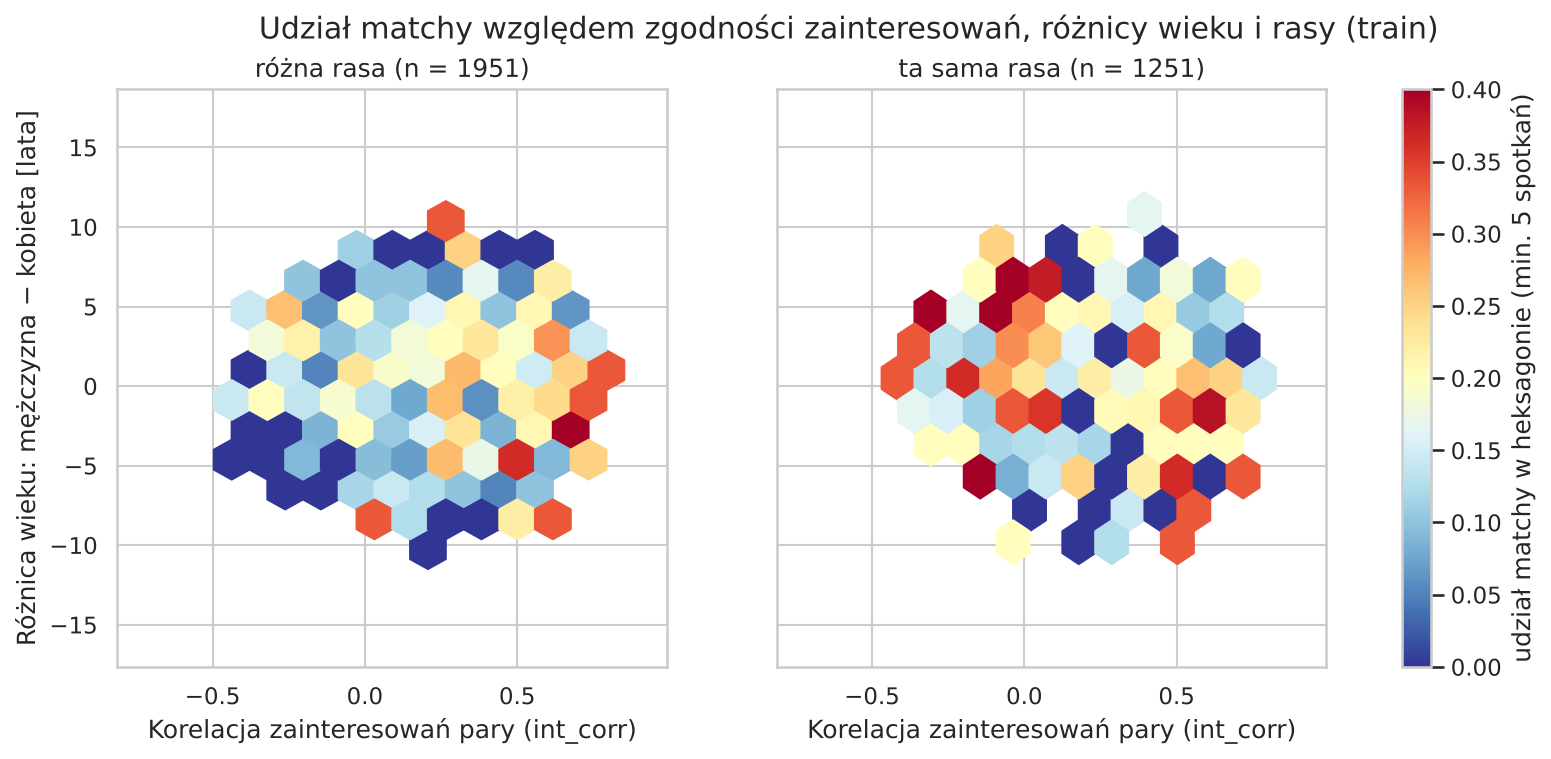
\includegraphics[width=\columnwidth]{../out/wykres_4_zmienne.png}
\caption{Udział matchy (kolor) względem podobieństwa zainteresowań (oś X),
różnicy wieku (oś Y) i~tego, czy para jest tej samej rasy (panele). Dane treningowe.}
\label{fig:4zm}
\end{figure}

\section{Przegląd literatury}
Fisman i~in.~\cite{fisman2006}, autorzy tych danych, badali, co wpływa na decyzję
pojedynczej osoby. Korzystali jednak z~ocen wystawianych już w~trakcie rozmowy,
więc ich wyniki nie przenoszą się wprost na przewidywanie przed spotkaniem.

Najbliższa mojemu zadaniu jest praca Joel i~in.~\cite{joel2017}. Na podobnych danych
z~ankiet przed speed datingiem modele uczenia maszynowego dobrze przewidywały, czy ktoś
jest ogólnie lubiany, ale prawie nie przewidywały sympatii konkretnej pary. Dlatego
słaby wynik mojego modelu jest spodziewany.

\section{Protokół eksperymentu}
\subsection{Podział i granica dopasowania}
Każda osoba ma 10--22 rozmowy w~jednym wydarzeniu. Gdybym podzielił wiersze losowo,
ta sama osoba trafiłaby do zbioru treningowego i~testowego, a model mógłby ,,zapamiętać''
ludzi zamiast się uczyć. Dlatego dzielę dane \textbf{po całych wydarzeniach}: każda
fala trafia w~całości do jednego zbioru (ziarno 42). Sprawdziłem, że train i~test nie
mają wspólnych uczestników.

\begin{itemize}
\item \textbf{Train:} \NTrain{} spotkań (16 fal) -- analiza danych i~uczenie.
\item \textbf{Validation:} 10 razy wydzielam z~train 20\% fal (ziarna 42--51)
i~na nich porównuję warianty.
\item \textbf{Test:} \NTest{} spotkań (fale 1, 2, 9, 16, 18) -- jedna ocena na końcu.
\end{itemize}

Uzupełnianie braków, skalowanie i~one-hot są dopasowywane tylko na części treningowej,
osobno w~każdym podziale (\texttt{Pipeline} ze scikit-learn).

\subsection{Metryka główna i miary pomocnicze}
Klasa pozytywna to match. Fałszywy alarm oznacza nietrafioną propozycję rozmowy,
a~przeoczenie -- pominiętą dobrą parę.

\noindent\textbf{Miara główna:} ROC AUC (im wyżej, tym lepiej; 0,5 = losowo). Mówi, czy model
stawia pary z~matchem wyżej niż pozostałe, niezależnie od progu decyzji.

\noindent\textbf{Miary pomocnicze:} F1 i~balanced accuracy przy progu 0,5 (czy model trafia
matche, nie ignorując rzadkiej klasy) oraz average precision (jakość rankingu przy
rzadkiej klasie). Accuracy podaję tylko informacyjnie.

\section{Preprocessing i baseline}
\textbf{Kolejność przetwarzania:}
\begin{enumerate}[leftmargin=*,itemsep=1pt]
\item usunięcie identyfikatorów, kolumn stałych, \NDuplikaty{} kolumn zapisanych
podwójnie (np.\ wiek partnera) i~kolumn z~ponad 60\% braków; dodanie różnicy wieku
i~zgodności kierunku studiów -- zostaje \NCech{} cech;
\item przeliczenie odpowiedzi punktowych na udziały (100 pkt);
\item cechy liczbowe: uzupełnienie braków, standaryzacja (dochód i~czesne przed
standaryzacją logarytmuję);
\item cechy nominalne: uzupełnienie najczęstszą wartością, one-hot.
\end{enumerate}

\textbf{Uzupełnianie braków.} Porównałem pięć metod: trzy proste (średnia, mediana,
najczęstsza wartość) i~dwie zaawansowane: KNN (wartość z~5 najbardziej podobnych osób)
oraz MICE (każda kolumna przewidywana regresją z~pozostałych). Na rysunku~\ref{fig:imp}
widać, że metody proste wstawiają wszędzie tę samą liczbę i~tworzą sztuczny ,,pik'',
a~KNN i~MICE lepiej zachowują kształt rozkładu.

\begin{figure}[H]
\centering
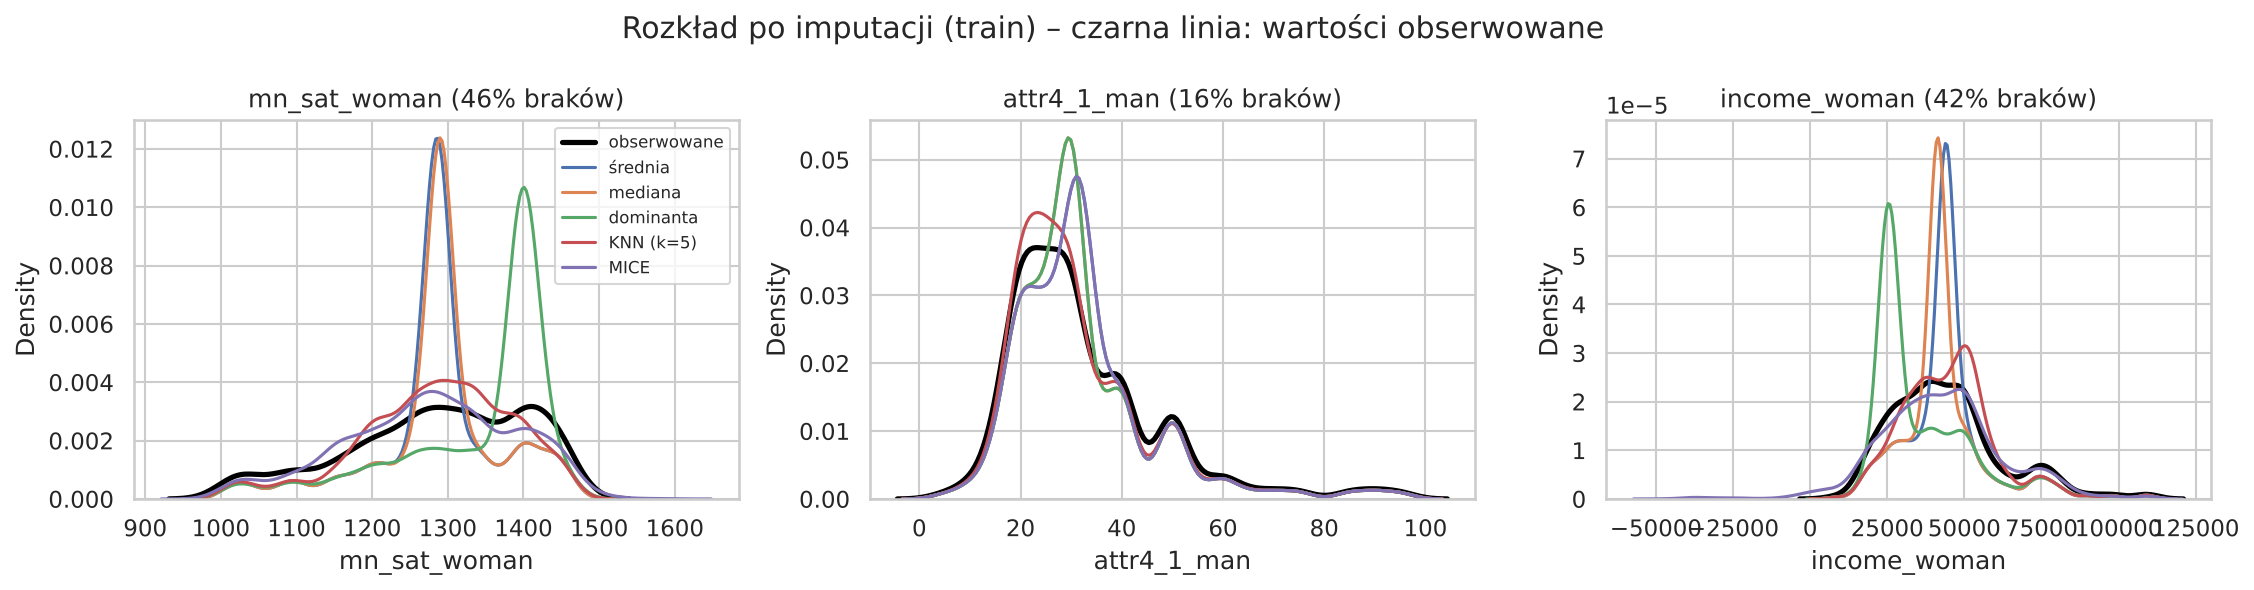
\includegraphics[width=\columnwidth]{../out/imputacja_rozklady.png}
\caption{Rozkład trzech kolumn po uzupełnieniu braków pięcioma metodami;
czarna linia -- prawdziwe (nieuzupełniane) wartości.}
\label{fig:imp}
\end{figure}

\textbf{Baseline.} Regresja logistyczna bez strojenia ($C=1$, wagi klas wyrównujące
rzadkość matchy). Porównuję ją z~modelem losowym (\texttt{DummyClassifier}).

\section{Wyniki etapu 1}
\textbf{Różne ziarna.} Tabela~\ref{tab:val} i~rysunek~\ref{fig:seeds} pokazują wyniki
na 10 podziałach walidacyjnych. Model jest wyraźnie lepszy od losowego. Metody
uzupełniania braków dają podobne wyniki: różnice między nimi są mniejsze niż różnice
między podziałami. Wynik zależy więc głównie od tego, które fale trafią do walidacji.
Las losowy uruchomiony z~10 różnymi ziarnami na jednym podziale zmieniał się mniej
(ROC AUC \ForestAucMean{} $\pm$ \ForestAucStd{}).

\begin{table}[H]
\centering
\caption{Walidacja (10 podziałów grupowych): średnia $\pm$ odchylenie standardowe.}
\label{tab:val}
\scriptsize
\setlength{\tabcolsep}{4pt}
\begin{tabular}{@{}lccc@{}}
\toprule
Imputacja & ROC AUC & AP & F1 (match)\\
\midrule
średnia & 0{,}588 $\pm$ 0{,}044 & 0{,}233 $\pm$ 0{,}036 & 0{,}298 $\pm$ 0{,}036\\
mediana & 0{,}588 $\pm$ 0{,}045 & 0{,}233 $\pm$ 0{,}038 & 0{,}301 $\pm$ 0{,}034\\
dominanta & 0{,}587 $\pm$ 0{,}044 & 0{,}231 $\pm$ 0{,}035 & 0{,}298 $\pm$ 0{,}037\\
KNN (k=5) & 0{,}603 $\pm$ 0{,}042 & 0{,}242 $\pm$ 0{,}040 & 0{,}308 $\pm$ 0{,}039\\
MICE & 0{,}592 $\pm$ 0{,}041 & 0{,}237 $\pm$ 0{,}042 & 0{,}309 $\pm$ 0{,}027\\
losowy (Dummy) & 0{,}512 $\pm$ 0{,}022 & 0{,}181 $\pm$ 0{,}014 & 0{,}195 $\pm$ 0{,}038\\
\bottomrule
\end{tabular}
\end{table}


\begin{figure}[H]
\centering
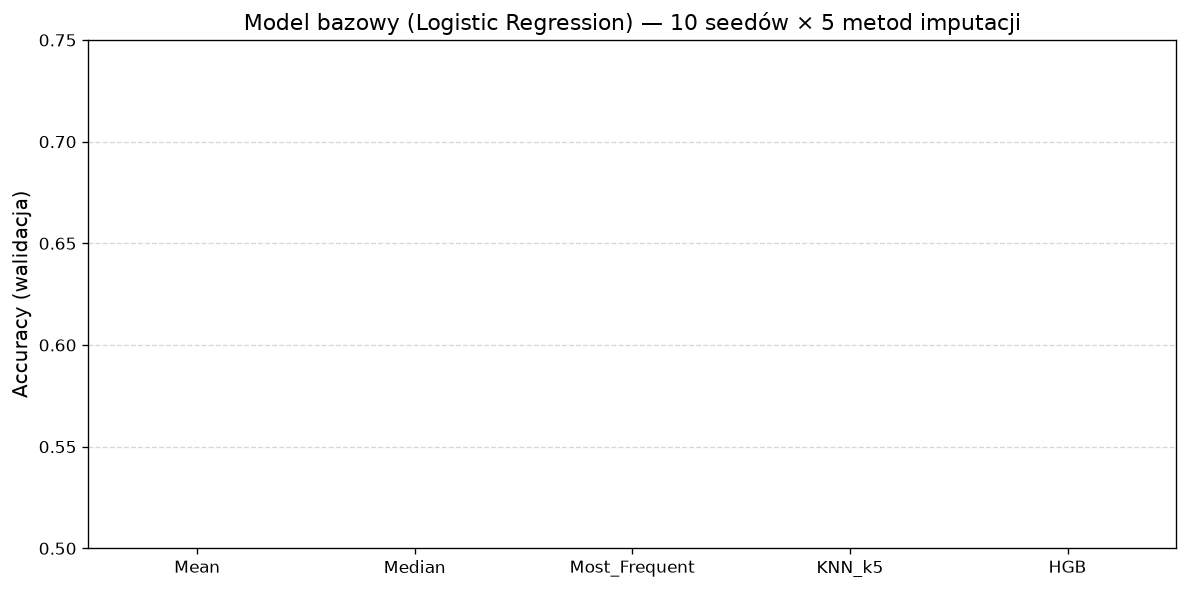
\includegraphics[width=\columnwidth]{../out/boxplot_seeds.png}
\caption{ROC AUC i~F1 na walidacji dla 5 metod uzupełniania braków i~modelu losowego
(10 ziaren).}
\label{fig:seeds}
\end{figure}

\textbf{Rozmiar zbioru treningowego.} Na rysunku~\ref{fig:lc} model był uczony na
10--100\% danych treningowych. Wynik walidacyjny rośnie z~\CurveFirst{} do ok.\ 0,59
przy 40\% danych i~dalej już nie rośnie. Wynik na danych treningowych jest dużo wyższy
(ok.\ 0,80), czyli model dopasowuje się do szczegółów danych treningowych. Więcej
danych niewiele pomoże; w~etapie~2 trzeba ograniczyć liczbę cech i~dodać regularyzację.

\begin{figure}[H]
\centering
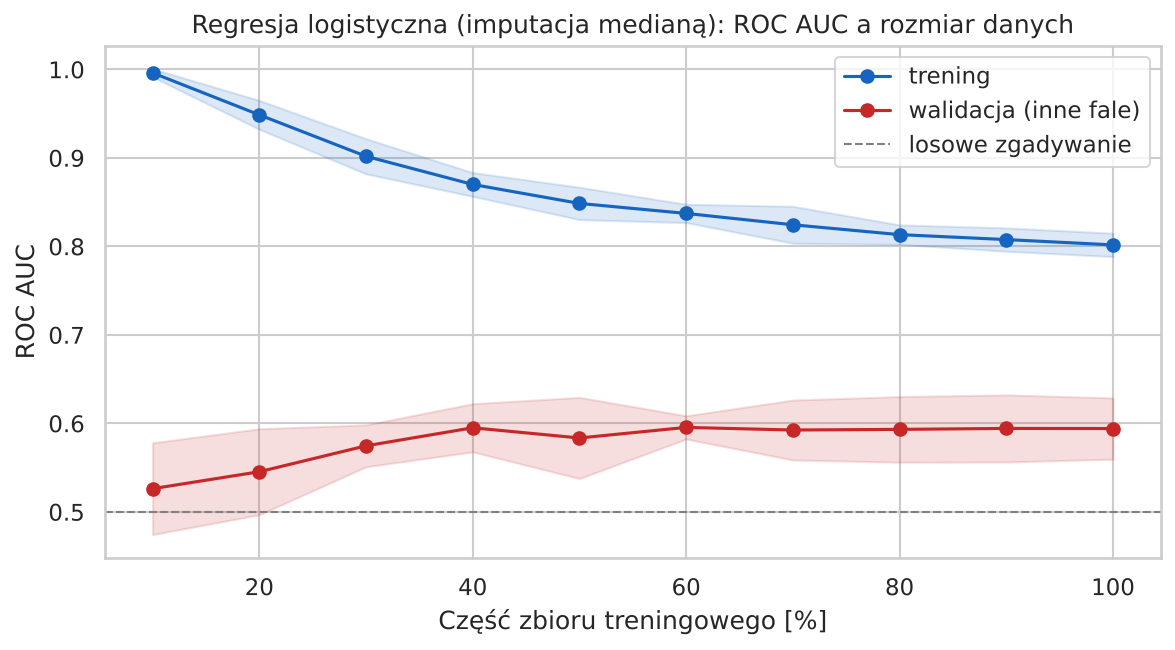
\includegraphics[width=\columnwidth]{../out/learning_curve.png}
\caption{ROC AUC w~zależności od części zbioru treningowego (5 podziałów).}
\label{fig:lc}
\end{figure}

\textbf{Test.} Model z~uzupełnianiem braków medianą (najprostsza z~metod, które
dawały podobny wynik), nauczony na całym train, uzyskał na teście ROC AUC = \TestAuc{},
F1 = \TestFone{} i~balanced accuracy = \TestBacc{}. Model losowy uzyskał ROC AUC \DummyAuc{}
i~F1 \DummyFone{}.

\textbf{Plan na etap 2:} strojenie regularyzacji i~wybór cech, modele nieliniowe
(las losowy, gradient boosting), cechy opisujące dopasowanie pary oraz dobór progu
decyzji.

\FloatBarrier
\bibliographystyle{plain}
\bibliography{bibliography}
\end{document}
